\chapter{Intersection cuts for submodular optimization}
\label{chap.submax}




\section{Introduction}


  In this chapter, we first consider $\cS$ as the Boolean-hypograph $\hyp_{\{0,1\}^n}(f)$ of $f$. We use convex extensions of $f$ in order to construct some $\cS$-free sets, which we call \textit{Boolean-hypograph-free}. The Boolean-hypograph set $\hyp_{\{0,1\}^n}(f)$ is a specialization of the constraint set $\{(x, t) \in \{0,1\}^n \times \bR: f_1(x) -f_2(x)  \ge \ell t\}$
with $ \ell \in \{0,1\}$. Then, we consider $\cS$ as this general constraint set and extend our results to handle this  general case. Finally, we propose an efficient algorithm to compute intersection cuts derived from $\cS$-free sets. To the best of our knowledge, intersection cuts have not  been applied directly to approximate problems with submodular and/or supermodular structures.

We implement intersection cuts within the \scip solver \cite{bestuzheva2021scip} and test them on \maxcut,  \pbm, and  \bdopt problems. We show the strengths and weaknesses of intersection cuts under these different settings.




\subsection{Literature review}

 
 
The \textit{base inequalities} \cite{nemhauser1978analysis} are a class of valid linear inequalities for the hypographs of general submodular functions. For a class of special submodular functions, lifting procedures  \cite{ahmed2011maximizing,shi2022sequence}  can strengthen the base inequalities. The  base inequalities can be separated either using heuristics \cite{ahmed2011maximizing} or a Benders-like framework \cite{coniglio2022submodular} if the point to be separated is integer. The method defined in \cite{Atamturk2021} combines valid inequalities for the submodular and supermodular components of an SS function. We refer to \cite{atamturk2020submodularity,atamturk2022supermodularity2,billionnet1985maximizing,bouhtou2010submodularity,han2022fractional,kilincc2021joint,rhys1970selection,shamaiah2010greedy,xusignomial,yu2023strong} for more details about the exploitation of  submodular/supermodular functions in mathematical programs. Supermodular polynomials in binary variables are defined and studied in \cite{billionnet1985maximizing,rhys1970selection}. The submodularity of the \dopt problem is exploited in \cite{SAGNOL2013258,shamaiah2010greedy}.


As already mentioned, intersection cuts generate valid inequalities for sets that are hard to optimize over. Gomory introduced the corner polyhedron \cite{gomory1969some}, and his celebrated mixed-integer cuts \cite{gomory1963algorithm} are special intersection cuts derived from split disjunctions \cite{Nemhauser1988}. The definition of intersection cuts for arbitrary set $\cS$ is due to \cite{dey2008,glover1973}. We refer to  \cite{andersen2010,andersen2007,basu2010,basu2019,conforti2015,conforti2011,cornuejols2015sufficiency,del2012relaxations,dey2008,richard2010group} for a more in-depth analysis.  The method given in \cite{towle2021intersection} can generate valid inequalities that cut off points outside $\cS$-free sets. We refer to \cite{andersen2007,belotti2015conic,klnc-karzan2015,kilinc-karzan2016,modaresi2015,modaresi2016} for relevant recent developments in mixed-integer conic programming.

For the cases where the nonconvexity of $\cS$ is not just due to integer variables, we refer to \cite{fischetti2018} for bilevel programs, \cite{bienstock2020outer} for outer-product sets, \cite{munoz2020maximal,munoz2022towards} for quadratic constraint sets, \cite{xusignomial} for signomial-term sets, and \cite{fischetti2020} for bilinear sets. The method given in \cite{serrano2019} constructs intersection cuts  for sets arising from factorable programs that contain DC functions \cite{khamisov1999optimization}.
 
 
Next, we discuss valid inequalities for polynomial programming, because we use polynomial programs in binary variables as a benchmark in our computational study. In \cite{bienstock2020outer}, intersection cuts approximate a nonconvex lifted set, namely the outer product set arising from  the extended formulation of a polynomial program. Lifted sets link decision variables to auxiliary variables representing (graphs of) monomials up to a given degree. We remark that in most combinatorial optimization problems,  decision variables are binaries. The polynomial program of interest is then a Boolean Multilinear Program (BMP).  The corresponding lifted set is the \textit{Boolean multilinear set} \cite{crama1993concave,fortet1960applications}, the convex hull of which is the so-called Boolean multilinear polytope. Valid inequalities for the Boolean multilinear polytope may be stronger than those for the  convex  hull of the outer product set. Various Gomory-Chvátal-based inequalities \cite{del2017polyhedral,del2018multilinear,del2020impact,del2022simple} are valid for the multilinear polytope. The separation and strength of these inequalities depend on  the hypergraph representing the underlying sparsity pattern of the multilinear set.

 We consider a constrained polynomial program, and assume that some  of its constraints are neither integrality constraints nor variable bound constraints. After lifting,  those constraints are linear and  thus define a convex set $\cS_1$. The lifted set $\cS_2$ is nonconvex, and $\cS_1 \not\subseteq \cS_2$.  The polynomial program is then equivalent to linear optimization over $\conv(\cS_1 \cap \cS_2)$. However, in general, $\conv(\cS_1 \cap \cS_2) \ne \cS_1 \cap \conv(\cS_2)$, so the convexification of the lifted set may not yield an equivalent convex problem. To address this issue, one attempt is to directly consider $\conv(\cS_1 \cap \cS_2)$ and generate valid inequalities for it.  Some work in this sense exists for certain interesting special cases, e.g.~the intersection of multilinear sets with additional constraint sets such as cardinality constraints \cite{chen2023multilinear}. Another attempt is to consider  constraints in projected formulations, \eg in mixed-integer quadratically constrained quadratic programs \cite{saxena2011convex}. Since the  representation complexity  of the projected formulation  is smaller than that of the  extended formulation, this approach is also amenable to computation. In \cite{chmiela2022implementation,munoz2020maximal}, intersection cuts for the set defined by a quadratic constraint are derived. If additionally, some of the nonbasic variables of the LP relaxation need to be integer, the monoidal technique \cite{ChmielaMunozSerrano2023} can strengthen such intersection cuts.

 
However, generating valid inequalities for Boolean multilinear constraints, and, more generally, constructing $\cS$-free sets for nonlinear constraints on discrete variables, remain problems of considerable interest. In this chapter, we look at these questions through a ``submodularity lens''.


\subsection{Contribution}
In \Cref{sec.freeforsub}, we already studied vairous properties for $\cS$-free sets arising in submodular maximization. We summarize those theoretical contributions here.
Our primary contribution is the construction of Boolean-hypograph-free sets. We show that a maximal Boolean-hypograph-free set $\cC \times \bR$ can be lifted from  a maximal $\{0,1\}^n$-free set.  We also give an alternative construction of Boolean-hypograph-free sets by exploiting  the submodularity. We relate the analytical properties of  $\bsF_{f}$ in \eqref{eq.bsf_f} to its combinatorial properties, which inherit those of the Lovász extension. We show that the epigraph $\epi(\bsF_{f})$ of $\bsF_{f}$ is a Boolean-hypograph-free set that is  larger than the epigraph of the Lovász extension. However, unlike in the continuous setting, $\epi(\bsF_{f})$ is not maximally Boolean-hypograph-free. We give necessary and sufficient conditions on maximal  Boolean-hypograph-free sets that contain $\epi(\bsF_{f})$.

The second contribution is  the computation of intersection cuts. We reduce the intersection cut separation problem to solving univariate nonlinear equations, which we achieve by a hybrid discrete Newton algorithm like \cite{Goemans}. We show that facets of $\epi(\bsF_{f})$ can be separated in strongly polynomial time. This implies that the (sub)-gradients required by the  Newton algorithm can be computed in a strongly polynomial time. The hybrid discrete Newton algorithm finds a zero point of a univariate nonlinear equation  in a finite number of steps. By contrast, the conventional bisection algorithm  only guarantees $\epsilon$-approximated solutions for $\epsilon > 0$.
 

Lastly, we  extend the previous findings to constraint sets involving an SS function. We show that any Boolean multilinear function is an SS function. This result yields intersection cuts for multilinear constraints in binary variables.


\subsection{Outline of the chapter}
The rest of the chapter is organized as follows. In \Cref{sec.app}, we consider applications for intersection cuts to Boolean multilinear constraints and \bdopt. In \Cref{sec.sep}, we propose the hybrid discrete Newton algorithm for computing intersection cuts. In \Cref{sec.cresult}, we analyze the computational results.


\section{Application}
\label{sec.app}
In this section, we discuss the application of intersection cuts to Boolean multilinear programming and D-optimal design. We exploit the submodular structures in these two problems.


\subsection{Boolean multilinear constraints}
\label{sec.bmc}
We consider the construction of $\cS$-free sets for Boolean multilinear constraints.
Since $x\in\{0,1\}\Leftrightarrow x^2=x$, one can reduce a  polynomial function defined on binary variables to a  multilinear  function, whose monomials do not include powers. For example, $x_1^2x_3^3+x_2^2$ can be reduced to $x_1x_3+x_2$.   A Boolean multilinear function is sometimes called a pseudo Boolean function.


 A similar case is the construction of $\cS$-free sets  for continuous quadratic constraints \cite{munoz2020maximal}. We call this construction the ``continuous approach''. It applies eigenvalue decomposition to factor the symmetric matrix representing quadratic terms in a quadratic constraint. Through this factorization, the quadratic constraint is reformulated to a DC constraint, possibly intersected with additional linear constraints. This reformulation is amenable to the reverse-linearization technique. Applying the technique with possibly additional operations, one can construct the so-called continuous-quadratic-free sets  \cite{munoz2020maximal} \footnote{The construction is \textit{de facto} discussed case by case. For some cases,  the reverse-linearization technique already suffices to produce continuous-quadratic-free sets. For other cases, one needs additional operations, \eg projecting out a lineality space. Notably, all cases require the eigenvalue decomposition and its resulting DC constraint.}. Multilinear terms, however, are represented by tensors. High-order tensor decomposition is  more complicated than matrix decomposition \cite{kolda2009tensor}. It is doubtful whether the continuous approach can be extended so as to produce DC functions from tensors.
 
Here we consider an alternative discrete approach. It exploits the submodularity and the supermodularity of Boolean multilinear functions. In \cite{billionnet1985maximizing,nemhauser1978analysis}, a class of Boolean multilinear functions is shown to be supermodular. We give a submodular-supermodular decomposition for general Boolean multilinear functions in the following.

\begin{proposition}
\label{lem.supml}
Consider a Boolean multilinear function $f: \cB \to \bR, x \mapsto \sum_{k \in [K]} a_k \prod_{j \in A_k}x_j$  with $K$ multilinear terms, where  $A_k \subseteq [n]$. Let $f = f_1 - f_2$ where
\begin{eqnarray}
    f_1(x) &:=& \quad \sum\limits_{k \in [K]\atop a_k < 0} a_k \prod\limits_{j \in A_k}x_j \label{prop9a}\\
    f_2(x) &:=& -\sum\limits_{k \in [K]\atop a_k > 0} a_k \prod\limits_{j \in A_k}x_j.\label{prop9b}
\end{eqnarray}
Then  $f_1,f_2$ are submodular over $\cB$.
\end{proposition}
\begin{proof}
It follows from Theorem 13.21 of \cite{crama2011boolean} that $f_1,f_2$ are submodular functions over $\cB$.\end{proof}


Since every Boolean multilinear function is an SS function, we can construct $\cS$-free sets for the corresponding Boolean-superlevel set or Boolean-hypograph set.

\begin{corollary}
\label{prop.bm}
Consider a  multilinear function $f: \cB \to \bR$, where $f(x) = \sum_{k \in [K]} a_i \prod_{j \in A_k}x_j$ for $A_k \subseteq [n]$ as in \Cref{lem.supml}, and $f_1(x),f_2(x)$ as in Eq.~\eqref{prop9a}-\eqref{prop9b}. 
%Let $f_1(x):=\sum_{k \in [K]\atop a_k < 0} a_k \prod_{j \in A_k}x_j$ and $f_2(x):=\sum_{k \in [K]\atop a_k > 0} -a_k \prod_{j \in A_k}x_j$.  
Let $\cS$, $\overline{\cS}$, and $\cC_{\relx{x}}$ be as \eqref{eq.cs}, \eqref{eq.csb}, \eqref{eq.c}, respectively. Then, the set $\cC_{\relx{x}}$ is an $\cS$-free set. Moreover, if $\relx{x} \notin \overline{\cS}$, then $\cC_{\relx{x}}$ does not contain $\relx{x}$ in its interior.
\end{corollary}
\begin{proof}
By \Cref{lem.supml}, we know that both $f_1$ and $f_2$ are submodular. Hence, the result follows by applying  \Cref{prop.dsfree}.
\end{proof}


Importing the notation in \Cref{lem.supml}, a BMP problem has the following form:
\begin{subequations}
\label{bmp}
\begin{alignat}{2}
	\max &&\quad t \\
&& \quad \sum_{k \in \cK_0} a_{ik} \prod_{j \in A_k}x_j &\ge  t  \label{bmp.obj}\\
  \forall i \in  [m] && \quad \sum_{k \in \cK_i} a_{ik} \prod_{j \in A_k}x_j & \ge 0  \label{bmp.cons}\\
  \forall  j \in [n] && \quad 	x_j  & \in \{0,  1\},
\end{alignat}
\end{subequations}
where $m$ is the number of constraints, $K$ is the number of  distinct multilinear terms in the BMP, $\cK_i \subseteq [K]$ is the index set of multilinear terms in the $i$-th constraint ($0$ for objective). Unconstrained BMP has several synonyms: \pbm  or \textsc{multilinear unconstrained binary optimization (MUBO)}.


To construct $\cS$-free sets for Boolean multilinear constraints in the BMP, we need to write them  as the standard form \eqref{eq.cs}.
For all $i \in [m]$ or $i = 0$, let $$f_i(x) := \sum_{k \in \cK_i} a_{ik} \prod_{j \in A_k} x_j,$$ and write $$f_i(x)= f_{i1}(x) - f_{i2}(x),$$ where $f_{i1}:= \sum_{k \in \cK_i:a_{ik} < 0} a_{ik} \prod_{j \in A_k} x_j$ and $f_{i2}:= -\sum_{k \in \cK_i:a_{ik} > 0} a_{ik} \prod_{j \in A_k} x_j$ are two  submodular functions.  

The objective and constraints of \eqref{bmp} can be represented as $$f_{i1}(x) - f_{i2}(x) \ge \ell_i t$$ (for all $i \in [m]$, $\ell_i = 0$, and $\ell_0$ = 1), which, by \Cref{prop.bm}, is in the standard form.  


Separating intersection cuts requires LP relaxations or simplicial cones.
 One can first lift multilinear terms to obtain an extended formulation:
 \begin{subequations}
\label{eq.bmplift}
\begin{alignat}{2}
	\max && \quad t\\
&& \quad \sum_{k \in \cK_0} a_{0k}  y_k &\ge  t  \label{bmplift.obj}  \\
  \forall i \in  [m] && \quad \sum_{k \in \cK_i} a_{ik}  y_k & \ge 0  \label{bmplift.cons}\\
	\quad  k \in [K] && \quad y_k &=  \prod_{j \in A_k}x_j \label{bmplift.monomial} \\
     \forall  j \in [n] && \quad 	x_j &\in \{0,  1\}
\end{alignat}
\end{subequations}

The standard Boolean linearization technique  \cite{crama1993concave} can reformulate a  multilinear term $\prod_{j \in A_k}x_j $ by  its underestimators and overestimators:
 \begin{subequations}
 \label{eq.stdlinear}
\begin{alignat}{2}
    \forall j \in A_k && \quad y_k  & \le x_j  \label{eq.stdlinear.over}\\
           		 && \quad  y_k  & \ge |A_k| + 1 - \sum_{j \in A_k} x_j \label{eq.stdlinear.under},
\end{alignat}
\end{subequations}
where $|A_k|$ is the cardinality of $A_k$. Then,  by linearizing each nonlinear constraint \eqref{bmplift.monomial}  as linear constraints in \eqref{eq.stdlinear}, one obtains a MILP reformulation of \eqref{eq.bmplift}.

To construct LP relaxations,  one can simply drop the integrality constraints $x_j \in \{0,1\}$. The direct LP relaxation of the MILP reformulation is also  an  LP relaxation of the BMP \eqref{eq.bmplift}. Following the method at the end of  \Cref{sec.maxsub},  we can construct an optimal tableau cone in the extended space $(x,y,t)$. The $\cS$-free set belongs to a projected space (\ie $(x,t)$-space). By extracting the $(x,t)$ entries of the rays of the optimal tableau cone, we  project the optimal tableau cone into the $(x,t)$-space. Given the projection of this optimal tableau cone, it is straightforward to construct intersection cuts for the BMP: we  separate the intersection cuts constructed by means of the $\cS$-free sets given by \Cref{prop.dsfree}.
 
As explained above, Boolean quadratic constraints belong to Boolean multilinear constraints, and continuous  quadratic constraints relax Boolean quadratic constraints. Both the continuous and discrete approaches can construct valid $\cS$-free sets for Boolean quadratic constraints. We remark that  maximal continuous-quadratic-free sets are no longer maximally Boolean-quadratic-free. It is easy to see that the  discrete approach  preserves the term-wise sparsity patterns of the SS functions and requires no factorizations. Therefore,  the  discrete approach is computationally amenable to ill-conditioned or sparse coefficient matrices.


\subsection{D-optimal design}
\label{sec.dopt}
In statistical estimation, optimal designs are a class of experimental designs that are optimal
with respect to some statistical criterion. We derive an extended convex MINLP  formulation for the \bdopt problem. In this formulation, the problem is a cardinality-constrained submodular maximization problem.



Let $\bS^m$ denote the set of $m$-by-$m$ symmetric matrices, and let $\bS^m_{+}$ (resp. $\bS^m_{++}$)  denote the set of $m$-by-$m$ positive semi-definite (resp. positive definite) matrices.
Given a set of  full row-rank matrices $\{M_j \in \bR^{m \times r_k}\}_{j \in  [n]}$, an
optimal design problem usually has the following form:
\begin{subequations}
\label{eq.optimal}
\begin{alignat}{2}
    \max  && \quad \Phi (\sum_{j \in  [n]}M_j \t{M_j} x_j )\\
      && \quad   \sum_{j \in [n]}x_j = k\\   
  \forall  j \in [n] && \quad     x_j  \in \{0,  1\},
\end{alignat}
\end{subequations}
where $k$ is the size of the design and $\Phi: \bS^m \to \bR$ is the design criterion. The matrix $M(x) := \sum_{j \in  [n]}M_j \t{M_j} x_j$ is called the \textit{information matrix}. For the D-optimal criterion \cite{bouhtou2010submodularity,sagnol2015computing}, $\Psi$ is  the log determinant function  $\ldet$.

Reseachers usually study \bdopt, where a statistical prior on the data $\{M_i\}_{i \in [n]}$ adds a regularization term $\epsilon I$  into the information matrix $M(x)$. Thus, $M(x) = \epsilon I + \sum_{j \in  [n]}M_j \t{M_j} x_j$. The additional term is also due to the well-posedness: when $x = 0$, we have that $\ldet(M(0)) = \ldet (\epsilon I) $ is well defined.
Then, the submodular maximization version of the \bdopt problem  has the following  formulation:
\begin{subequations}
\label{eq.optimal2}
\begin{alignat}{2}
    \max  && \quad \ldet \left(\epsilon I + \sum_{j \in  [n]} M_j \t{M_j} x_j  \right) \\
      && \quad   \sum_{j \in [n]}x_j = k\\   
  \forall  j \in [n] && \quad     x_j  \in \{0,  1\},
\end{alignat}
\end{subequations}

The log determinant function is concave and has a semi-definite programming (SDP) and geometric programming representation \cite{aps2018mosek}.  The scalability 
 of the mixed-integer log determinant formulation above is limited by the current state of SDP solvers. Based on the second order cone representation of the determinant function $\det(M(x))$ \cite{sagnol2015computing}, we give an extended formulation for \eqref{eq.optimal2}:
\begin{subequations}
\label{ref.dopt}
  \begin{alignat}{2}
   	 \max \quad &&  t  \\
  	 \quad && t \le \sum_{i \in [m]} \log(J_{ii})  \label{ref.log}\\
      \quad && \sum_{j \in [n] \cup \{0\}} M_j Z_j  = J \\
  	 \quad &&  J \textup{ is lower triangular} \\
  	 \quad  j \in [n] \cup \{0\} \, i \in [m] &&\norm{Z_j e_i}^2 \le u_{ji} x_j  \label{ref.soc}\\
      \quad i \in [m] &&  \sum_{j \in [n] \cup \{0\}} u_{ji} \le J_{ii}\\
      \quad && \sum_{j \in [n]} x_j = k \\
   		 \quad  && x \in \{1\} \times \cB  \\
       		 \quad &&  J \in \bR^{m \times m}\\
      \quad  j \in [n] \cup \{0\} && Z_j \in \bR^{r_j \times m}\\
      \quad j \in [n] \cup \{0\} \, i \in [m] &&  u_{ji} \in \bR_+^{r_j \times m},
  \end{alignat}
\end{subequations}
where  $M_0 = \epsilon^{1/2}I$ is an auxiliary matrix.
One can represent this formulation by low-dimensional convex cones \cite{aps2018mosek}, \eg (rotated) second-order cones, and exponential cones. Therefore, this extended formulation is amenable to computation.


\begin{proposition}
\eqref{ref.dopt} is equivalent to \eqref{eq.optimal2}, and the objective function of \eqref{eq.optimal2} is submodular w.r.t. $x$.
\end{proposition}
\begin{proof}
One can modify the original D-optimal design problem by adding a slack variable $x_0 = 1$.
Applying the logarithmic transformation to results in \cite{sagnol2015computing}, \eqref{ref.dopt} is equivalent to \eqref{eq.optimal2}.  It follows from  \cite{SAGNOL2013258,shamaiah2010greedy} that \eqref{eq.optimal2} is submodular w.r.t. $x$.
\end{proof}

A global optimization solver like \scip can linearize the constraints in the extended formulation \eqref{ref.dopt}, and thus produces an LP relaxation in the extended space. We can  obtain an optimal tableau cone as the approach dealing with the BMP. Then, we can construct intersection cuts from  Boolean-hypograph-free sets.


 
 
\section{Separation problem}
\label{sec.sep}
In this section,  we consider the separation problem for an intersection cut from an $\cS$-free set. Summarizing the previous sections, the $\cS$-free set is in the  form of $$
    \cC := \{(x,t) \in \bR^n \times \bR: \mathsf{G}(x) \le \ell t\},
$$
where  $\mathsf{G}(x) = \max_{s \in \ext(\ep{g})} sx$ is the extended envelope of some submodular function $g$ over $\cB$ and $ \ell \in \{0, 1\}$. We remark that the extended envelope epigraph $\ee{f}$ in \eqref{eq.ee} is a special case with $ \ell = 1$ and $g=f$; the set $\cC_{\relx{x}}$ in  \eqref{eq.c} is also a special case that $g(x)= f_1(x) - \gamma^\ast x$.

Assume that $z^\ast:=(\relx{x}, \relx{t})$ is the vertex of an optimal tableau cone $\cR$, and $z^\ast \in \inter(\cC)$. Recalling the cut coefficient formula in \Cref{sec.premic}, the separation problem consists in computing the step length along each ray $r^j$:
\begin{equation}
\label{eq.supstep}
\eta_j^\ast = \sup_{\eta_j \ge 0}\{\eta_j: z^\ast + \eta_j r^j \in \cC\}.   
\end{equation}
This line search problem asks for the step length to the border of $\cC$ along the ray $r^j$ from $z^\ast$ which, we recall, is an interior point of $\mathcal{C}$.   We denote by $r^j_x, r^j_t$ the projection of $r^j$ on $x$- and $t$- spaces. Looking at the function defining $\cC$, the intersection step length $\eta_j^\ast$ is the zero point of the following function:
$$\zeta^j:\bR_+ \to \bR, \textup{ where } \zeta^j(\eta_j) = \ell  (\relx{t} + r^j_t \eta_j) -  \mathsf{G}(\relx{x} + r^j_x  \eta_j ).$$
This function enjoys the following properties.

\begin{proposition}
\label{prop.uni}
$\zeta^j$ is a  concave  piece-wise linear function over  $[0,+\infty]$ with  $\zeta^j(0) > 0$.  If $\eta^\ast_j < \infty$ and there exists an $\eta'_j > 0$ with $\zeta^j(\eta'_j) = 0$, then $\eta'_j = \eta^\ast_j$, \ie the solution $\eta^\ast_j$ must be unique.  For all $s^\ast \in \argmax_{s \in \ext(\ep{g})} s (\relx{x}+\eta_j r^j_x)$, $\ell r^j_t- s^\ast r^j_x$ is a subgradient in $\partial \zeta^j( \eta_j)$. For $\eta_j > \eta^\ast_j$, $\partial \zeta^j( \eta_j) \le \partial \zeta^j( \eta^\ast_j)$.
\end{proposition}
\begin{proof}
Since  the extended envelope $\mathsf{G}$ is the maximum of linear functions, it is convex and piece-wise linear, so  $\zeta^j$ is concave and piece-wise linear. Since $\zeta^j(0) = \ell \relx{t} - \mathsf{G}(\relx{x})$, it follows from the assumption $z^\ast \in \inter(\cC)$ that $  \ell \relx{t} >   \mathsf{G}(\relx{x})$ and thus  $\zeta^j(0) > 0$. Since $\cC$ is closed and convex, $\eta'_j = \eta^\ast_j$ if and only if $z^\ast + \eta'_j r^j  \in \bd(\cC)$. That is $\mathsf{G}(r^j_x \eta_j + \relx{x}) = \mathsf{G}(\relx{x}) + r^j_t \eta'_j $, i.e., $\zeta^j(\eta'_j) = 0$. Since $s^\ast \in \partial {\mathsf{G}}(\relx{x}+  r^j_x \eta_j)$, by the chain rule, $\ell r^j_t - s^\ast r^j_x$ is a subgradient of $\zeta^j$. By the concavity of $\zeta^j$, its subgradients are non-increasing.
\end{proof}


 By \Cref{prop.uni}, the line search problem \eqref{eq.supstep} is reduced to solving the univariate nonlinear equation:
\begin{equation}
\label{eq.nleq}
	\zeta^j(\eta^j) = 0.
\end{equation}
For each ray $r^j$, solving \eqref{eq.nleq} gives the unique zero point of the univariate function $\zeta^j$, or certifies that no such point exists.



To solve the univariate nonlinear equation \eqref{eq.nleq}, it is natural to deploy a Newton-like algorithm. Therefore, we need the value and (sub)gradient information of $\zeta^j$: the  computation of $\zeta^j$ can then be reduced to the  computation of $\mathsf{G}$. The value and subgradients of $\mathsf{G}$ are obtained by means of a sorting algorithm (see \Cref{prop.out}). We note that these computations can be carried out in strongly polynomial time.  

Previous works \cite{ChmielaMunozSerrano2023,xusignomial} use the bisection algorithm, which guarantees finding the zero point within a given tolerance. Our implementation, which we call \textit{hybrid discrete Newton algorithm}, is  a combination of the discrete Newton algorithm \cite{Goemans} and the bisection algorithm. The role of the bisection algorithm in Alg.~\ref{algo.newton} is to help find a starting point for the Newton algorithm. Thanks to the piece-wise linearity of the univariate function $\zeta^j$, our algorithm finds an exact zero point in a finite time.

\begin{algorithm}[htbp]
 \textbf{Input:} The univariate function $\zeta^j$, (scalar) starting  point $\Delta > 0$ (default: 0.2), a numeric $\eta_{\infty}$ representing $+\infty$, and the maximum number $I$ of search steps (default: 500)\;
 \textbf{Output:}  $\eta_j > 0$ such that $\zeta^j(\eta_j) = 0$\;
 Let step number $i = 0$, and let step length $\eta_{j}  =\Delta$\;
 \uIf{$\zeta^j(\eta_\infty) > 0$}{
    $\eta_j = \eta_\infty$\Comment*[r]{safeguard}
 }
 \Else{
 \While{$i < I$}
 {
Let $ s^\ast \in \argmax_{s \in \ext(\ep{g})} s (\relx{x}+ r^j_x \eta_j)$\;
Compute a subgradient $\beta =r^j_t - s^\ast r^j_x$\;
\uIf{$\zeta^{j}(\eta_j) = 0$}{
\Break\;
}
\ElseIf{$ \beta < 0$}{
$\eta_j = \eta_j - \frac{\zeta^j(\eta_j)}{\beta}$ \Comment*[r]{Newton step}\label{algo:newton.step}
}
\Else{
$\eta_j = 2 \eta_j$\Comment*[r]{bisection step}\label{algo:bis.step}
}
$i = i +1$\;
 }}
\caption{Hybrid discrete Newton algorithm}
\label{algo.newton}
\end{algorithm}




\begin{proposition}
\label{prop.converg}
The hybrid discrete Newton algorithm terminates in a finite number of steps and finds the zero point $\eta^\ast_j$.
\end{proposition}
\begin{proof}
For all $\eta \in \bR_+$, we assume that  \Cref{algo.newton} chooses and computes a unique subgradient $\beta$ at $\eta_j$,  we denote it  $\nabla \zeta^j(\eta_j)$, and call it algorithmic gradient.
The concavity of $\zeta^j$ implies that its algorithmic gradient is monotone-decreasing w.r.t. $\eta_j$. There is a threshold $\eta'_j \ge 0$ such that, for all $\eta_j \in [0, \eta'_j)$, the algorithmic gradient $\nabla\zeta^j(\eta_j) > 0$; for all $\eta_j \in  [\eta'_j, +\infty]$ (called the Newton step region), the algorithmic gradient $\nabla\zeta^j(\eta_j) \le  0$.

After a finite number of bisection steps (at most $\lceil \log(\eta'_j / \Delta)\rceil$), the algorithm enters the Newton step region $[\eta'_j, +\infty]$, where the algorithmic gradient is always negative.
Then, we prove that the algorithmic gradient $\nabla\zeta^j(\eta_j)$ at step $i$ is different from that at step $i-1$, and the algorithm stays in the  Newton step region. Since $\zeta^j$ is piece-wise linear (the number of its distinct algorithmic gradients is finite),  the algorithm must terminate in a finite number of steps.

If at step $i-1$, $\zeta^j(\eta_j -  \frac{\zeta^j(\eta_j)}{\nabla\zeta^j(\eta_j)}) = 0 $, then the algorithm terminates at this step and finds the zero point. If at step $i-1$, $\zeta^j(\eta_j - \frac{\zeta^j(\eta_j)}{\nabla\zeta^j(\eta_j)}) < 0 $, then we prove that $\nabla \zeta^j(\eta_j - \frac{\zeta^j(\eta_j)}{\nabla\zeta^j(\eta_j)}) \ne \nabla \zeta^j(\eta_j)$ and $\nabla \zeta^j(\eta_j - \frac{\zeta^j(\eta_j)}{\nabla\zeta^j(\eta_j)}) \le 0$.

First, assume, to aim at a contradiction, that $\nabla \zeta^j(\eta_j - \frac{\zeta^j(\eta_j)}{\nabla\zeta^j(\eta_j)}) = \nabla \zeta^j(\eta_j)$.  Knowing that the algorithmic gradient is  monotone-decreasing, the piece-wise linearity of  $\zeta^j$ implies that this algorithmic gradient is constant in the range $[\eta_j -  \frac{\zeta^j(\eta_j)}{\nabla\zeta^j(\eta_j)}, \eta_j]$. It follows that for all $\delta \in [0, \frac{\zeta^j(\eta_j)}{\nabla\zeta^j(\eta_j)}]$, $\zeta^j(\eta_j - \delta) = \zeta^j(\eta_j) - \delta   \nabla\zeta^j(\eta_j)$. Hence, $\zeta^j(\eta_j - \frac{\zeta^j(\eta_j)}{\nabla\zeta^j(\eta_j)}) = 0$, which leads to a contradiction.

Second, we show that $\nabla \zeta^j(\eta_j - \frac{\zeta^j(\eta_j)}{\nabla\zeta^j(\eta_j)}) \le 0$. When $\frac{\zeta^j(\eta_j)}{\nabla\zeta^j(\eta_j)} \le 0$, by the mononcity of $\nabla \zeta^j$, $\nabla \zeta^j(\eta_j - \frac{\zeta^j(\eta_j)}{\nabla\zeta^j(\eta_j)}) \le \nabla \zeta^j(\eta_j) < 0$. When $\frac{\zeta^j(\eta_j)}{\nabla\zeta^j(\eta_j)} > 0$, as by assumption that $\nabla\zeta^j(\eta_j) < 0$, $\zeta^j(\eta_j)$ must be negative. Then, by the concavity of $\zeta^j$, $\zeta^j(\eta_j - \frac{\zeta^j(\eta_j)}{\nabla\zeta^j(\eta_j)}) \le \zeta^j(\eta_j) - \nabla\zeta^j(\eta_j)\frac{\zeta^j(\eta_j)}{\nabla\zeta^j(\eta_j)} = 0$. This implies that $\nabla \zeta^j(\eta_j - \frac{\zeta^j(\eta_j)}{\nabla\zeta^j(\eta_j)}) \le 0$.
\end{proof}
From \Cref{prop.converg},  the hybrid discrete Newton algorithm first executes bisection steps with increasing $\eta_j$ and $\zeta^j(\eta_j)$. Then it enters into the Newton step region. After a single Newton step, $\zeta^j(\eta_j)$ becomes negative, and then monotonically increases to zero in a finite number of steps. 

The discrete Newton algorithm in \cite{Goemans} is applied to the line search problem for submodular polyhedra, which are polars of extended polymatroids. In that context, it runs in a strongly polynomial time. In our case, $\cC$ contains the extended polymatroid, but it is unbounded in general. The corresponding line search problem may have no solutions, if the  ray  $r^j$ is contained in the recession cone of $\cC$. Therefore, \Cref{algo.newton} needs a safeguard step, where we evaluate $\zeta^j$ at a user-defined infinity. One may also prove that \Cref{algo.newton} runs in a strongly polynomial time, but a careful analysis for the unbounded case is needed. 

\section{Computational results}
\label{sec.cresult}
In this section, we conduct computational experiments to test the proposed cuts. The source code, data, and detailed results can be found in our online repository: \href{https://github.com/lidingxu/Subcut}{github.com/lidingxu/Subcut}.


\textbf{Setup and performance metrics.}  The experiments are conducted on a server with  Intel Xeon W-2245 CPU @ 3.90GHz and 126GB main memory. We use \scip 8.0 \cite{bestuzheva2021scip} as a MINLP framework to solve the natural  formulations of test problems.  \scip is equipped with \texttt{CPLEX} 22.1 as an LP solver, and \texttt{IPOPT} 3.14 as an NLP solver.


By \Cref{thm.bin}, the simple lifted split $H_j := \{x \in \bR^n: 0 \le x_j \le 1\} \times \bR$ is a maximal $\hyp_{\cB}(f)$-free set,  where the splitting variable $x_j$ is chosen as the most fractional entry of the relaxation solution. We have three settings of  cut separation routines (cut separators). The \textit{submodular cut} (resp. the \textit{split cut}) setting  adds intersection cuts derived from  $\ee{f}$ (resp. $H_j$), and the \textit{default} setting does not add any intersection cuts. Our separators adhere to unified parameter settings that aim to maximize the likelihood of \scip invoking our separators.  These parameters for the cut separators in \scip are detailed in \cite{BibEntry2023Jul}. Notably, during our experiments, we observed that the cut separators are predominantly influenced by the following parameters:

\begin{itemize}
    \item SEPA\_PRIORITY: the priority of the intersection cut separator. We  set it to 100000 (the separators are called in a predefined order, which is given by the priorities of the separators).
    \item SEPA\_DELAY: the default for whether the separation method should be delayed, if other separators found cuts. We set it to TRUE, \ie delayed. (If the separator's separation method is marked to be delayed, it is only executed after no other separator  found a cut during the price-and-cut loop).
    \item SEPA\_MINVIOL: the minimal violation a cut must fulfill such that the cut can be added. We set it to $10^{-4}$.
    \item SEPA\_NCUTSLIMITROOT: the limit for the number of cuts generated at the root node. We  set it to -1, meaning that the separation is unlimited.
\end{itemize}

 Most cut separators in \scip have priorities lower than 15, leading us to assign the highest priority to our cut separators. Consequently, \scip calls our cut separators before the others during the optimization process.

The proposed cuts in this chapter are represented by the expression $\alpha x + \mu t \leq \beta$. When constructing a cut of this form to separate a point $(\relx{x}, \relx{t})$, it is considered numerically \emph{ill-conditioned}, if the condition number $\max(\alpha, \mu) / \min(\alpha, \mu)$ becomes too large.

The objective of the proposed cuts is to approximate the constraint $f(x) \geq \ell t$, where $f$ represents either a submodular function or an SS function. During our analysis, we observed that the magnitude of $f(x)$ can be significantly larger than 1. For submodular cuts, this leads to a numerically ill-conditioned cut, where the magnitude of $\mu$ is much smaller than the magnitudes of the entries in $\alpha$.

A similar issue arises in the numerical optimization of finite sums of nonlinear functions, such as problems of the form $\min g(x):= \min \sum_{j \in [k]} g_j(x)$. To enhance numerical stability during optimization, it is more favorable to optimize the average $g(x)/k$ rather than $g(x)$ itself. Therefore, we adopt a similar pre-processing step to scale our test problems.

Specifically, we scale the constraint $f(x) \geq \ell t$ into $f(x) / \chi \geq \ell t$, where $\chi$ represents a positive scaling factor. The purpose of this step is to ensure that the magnitude of $\mu$ becomes similar to that of $\alpha$ and $\beta$. The factor $\chi$ is selected as follows:

\begin{itemize}
    \item For \maxcut problems, $\chi$ is the number of edges of the graph.
    \item For \pbm problems, $\chi$ is the number of  degree-4 monomials in the polynomial.
    \item For \dopt problems, $\chi$ is 1.
\end{itemize}


 \scip has internal routines of higher authority than any individual cut separator. These routines  can control whether to invoke a cut separator and whether to apply the cuts found by the separator. Interfaces of these routines are not exposed publicly, but  \scip  allows us to affect these routines through the parameters of cut separators.  Therefore, we conduct the above three settings
 respectively in two distinct  configurations: the \textit{standalone}  and the \textit{embedded} configurations. 
 
 In the \textit{standalone}  configuration, we aim at measuring the  performance of our cuts in a ``clean'' environment without interacting with other cuts, so we deactivate all of \scip's internal cut separators.  In the \textit{embedded} configuration, we aim at measuring the  performance of our cuts in a ``real'' environment. According to Example 6.10 of \cite{conforti2014integer}, our split cuts correspond to Gomory mixed integer cuts.  To ensure a fair comparison, we require an equal level of implementation for intersection cuts, including the data structure and parameter settings. Hence, we replace \scip's implementation of Gomory mixed integer cuts with our own implementation, thereby disabling \scip's internal Gomory mixed integer cut separators in the embedded configuration.

 We focus on  the root node performance and measure the \textit{closed root gap}. Let $d_1$ be the value of the first LP relaxation (without cuts added), let $d_2$ be the dual
bound  after all the cuts are added, and  let $p$ be a reference primal bound. The closed root gap $(d_2-d_1) /(p-d_1)$
 is the closed gap improvement of $d_2$ with
respect to $d_1$.  We also record the number of added cuts, the relative improvement to the default setting, and the total running time. For each configuration and setting,  we compute these statistics' shifted geometric means (SGMs) with a shift of 1 over our test sets.

For each of the following experiments, we present and analyze computational results in the form of tables and scatter plots. The tables contain SGMs of the statistics, including the closed root gap (abbreviated as ``closed''), the total running time (abbreviated as ``time''), and the number of applied cuts  (abbreviated as ``cuts'').  Moreover, the ``relative'' column  displays the relative value of the closed root gap of one configuration that our cuts are enabled   to that of the default configuration. Thus, the ``relative improvement'' due to our cuts is defined as the ``relative'' minus one. The scatter plots compare the closed root gap of each instance between two different settings. Furthermore, each scatter plot indicates the number of instances where one setting outperforms the other, referred to as ``win'' instances.

\bigskip

\noindent\textbf{Experiment 1:} \maxcut. Consider an undirected graph $G=(V,E,w)$, where $V$ is the set of nodes, $E$ is the set of edges, and $w$ is a weight function over $E$. For a subset $S$ of $V$, its associated cut capacity  is  the sum of the weights of edges with one end node in $S$ and the other end node  in $V \setminus S$. The \maxcut problem aims at finding a subset $S \subseteq V$ with  maximum cut capacity. Let $V = [n]$, and we use a  binary variable vector $x \in \cB$ indicating whether vertices belong to $S$.  The problem can be formulated as the following   quadratic unconstrained binary optimization (QUBO) problem: $$
    \max_{x \in \cB}  \sum_{\{i, j\} \in E}w_{ij} ((1-x_i)x_j + x_i(1-x_j)).$$
 When $w$ is nonnegative, the cut capacity function (the objective function) is  submodular. 

The Biq Mac library  \cite{wiegele2007biq} offers a collection of  \maxcut and QUBO instances of medium size.
 Our benchmark consists of two sub-benchmarks with 30 ``g05'' and respectively 30 ``pw'' \maxcut instances with nonnegative weights from the library. These instances are generated randomly by Giovanni Rinaldi's \texttt{rudy} code \cite{rendl2010solving,rinaldi1998rudy}.  For each dimension $n=60,80,100$, the ``g05'' sub-benchmark consists of 10 unweighted graphs with edge probability 0.5. For each graph density in $\{0.1,0.5,0.9\}$,   the ``pw'' sub-benchmark consists of 10 graphs with integer edge weights chosen from $[0,10]$. 
 
The reference primal bounds are also from the Biq Mac library. We encode the hypograph reformulation \eqref{eq.milp} of the QUBO. \scip will automatically reformulate the problem into a MILP via the reformulation-linearization technique  (RLT) \cite{adams1986tight}. This MILP formulation is a special case of the extended formulation \eqref{ref.dopt} of a degree-2 BMP with $m = 0$.
 
 
For the standalone  configuration, the relative improvement of submodular cuts is $342\%$  compared to $178\%$  of split cuts. In the standalone configuration, we can compare the ``clean'' strengths of intersection cuts derived from different Boolean-hypograph-free sets. As observed from the scatter plots in  \Cref{fig:mubo}, the submodular cut setting outperforms the split cut setting in 42 instances under the standalone configuration.  Although split cuts are derived from maximal Boolean-hypograph-free sets and submodular cuts are derived from non-maximal ones, the clean performance of  split cuts is worse.  Regarding the embedded configuration,  the relative improvement of submodular cuts is $85\%$,  compared to $58\%$   of split cuts. The scatter plot shows that the submodular cut setting surpasses the split cut setting in 34 instances under this configuration.
 
We observe that fewer split cuts are generated than submodular cuts. This means that the efficiency of some split cuts does not satisfy \scip's internal criteria, so \scip abandons more split cuts  than submodular cuts.  As two types of cuts are derived using the same principle but from different Boolean-hypograph-free sets,  the distances between the relaxation points to the boundary of Boolean-hypograph-free sets determine the cut efficiency. This observation suggests that relaxation points are further from the boundary of the extended envelope epigraph than from the splits. The separation time of split cuts is shorter than that of submodular cuts, particularly for the ``pw'' instances with a high graph density (0.9). This is because separating submodular cuts requires solving  nonlinear equations that involve sorting and computing graph cuts, while the split cuts can be computed  in a closed form.

\begin{table} [htbp]
\centering
\scalebox{0.85}{
\begin{tabular}{c|cr|cccr|cccr}
\toprule
\multirow{2}{*}{\texttt{Configuration}} &
\multicolumn{2}{c|}{\texttt{Default}}    &
\multicolumn{4}{c|}{\texttt{Submodular cut}} &
\multicolumn{4}{c}{\texttt{Split cut}} 	 \\
 & closed & time & closed & relative & time & cuts & closed & relative & time & cuts\\
\hline
standalone & 0.026 & 4.33 & 0.111 & 4.418 & 22.9 & 215.48 &  0.075 & 2.78 & 7.04 & 75.04\\
embedded&   0.097 & 4.77 & 0.161 & 1.852 & 68.19 & 162.5 &  0.139 & 1.575 & 9.4 & 67.6 \\
\bottomrule
\end{tabular}}
\caption{Summary of \maxcut results}\label{alpha}
\end{table}

\begin{figure}[h]
    \centering
    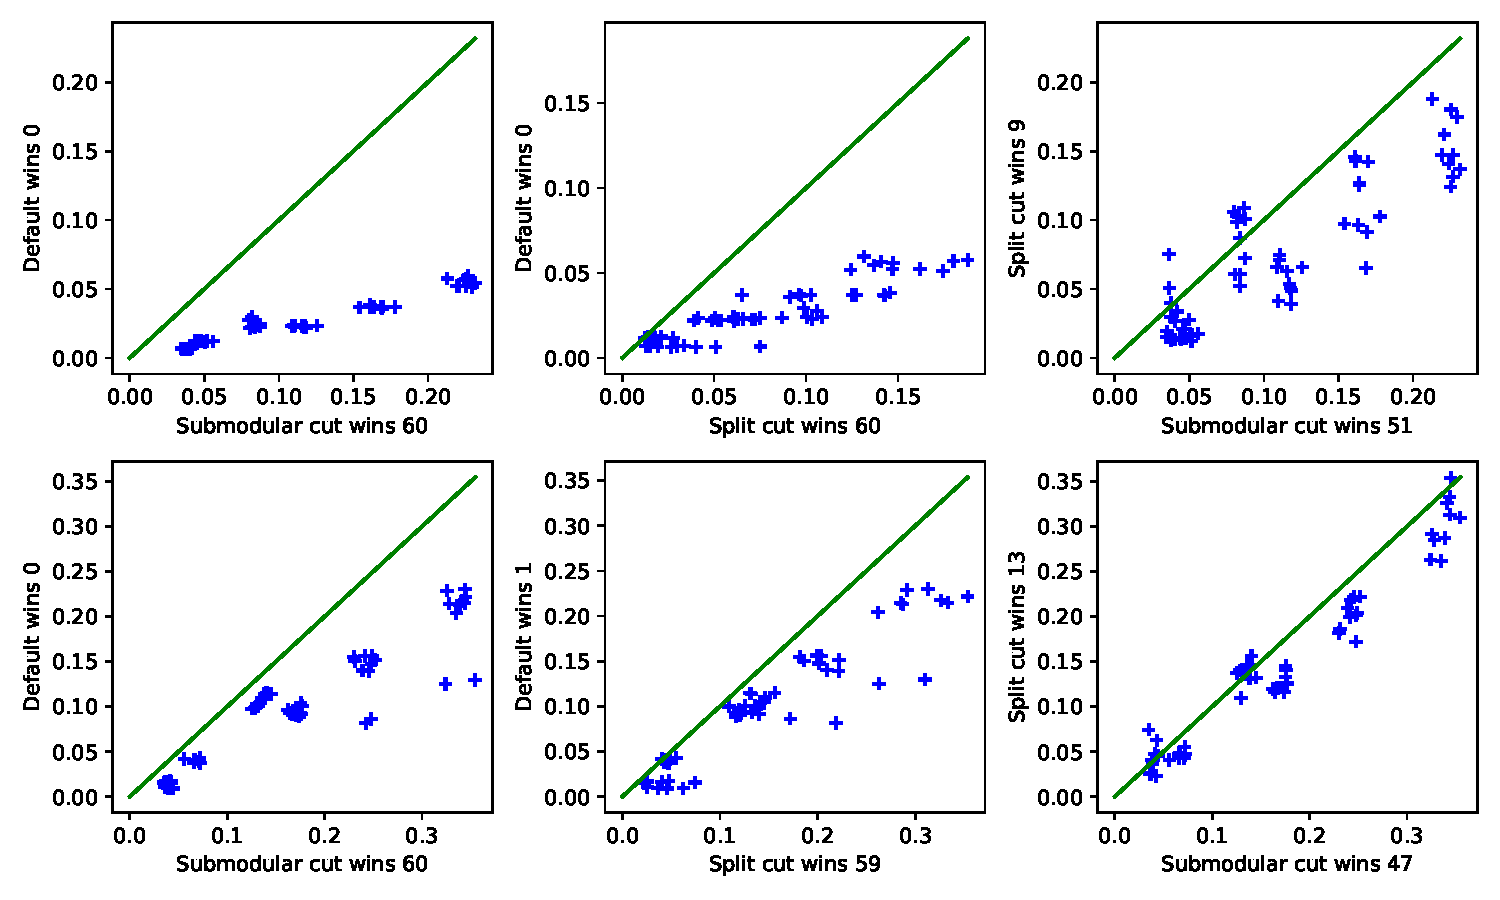
\includegraphics[width=0.99\textwidth]{Chaptersub/media/scatter_qubo.pdf}
    \caption{Scatter plots of \maxcut results in standalone (top) and embedded (bottom) configurations}
    \label{fig:qubo}
\end{figure}

%\bigskip

\noindent\textbf{Experiment 2:} \pbm.
As  mentioned, \pbm is a MUBO problem, a generalization of QUBO. We can use techniques from \Cref{sec.ss} to generate intersection cuts.   


POLIP \cite{Ulriks} is a library of polynomially constrained
mixed-integer programming instances. All MUBO instances in  POLIP with degree higher than 2 are 41 ``autocorr\_bern'' instances,  which are also included in MINLPLib \cite{minlplib,Vigerske2022Feb}.
These instances arise from short ranged non-disordered lattice spin model (the Bernasconi model) \cite{liers2010non} in theoretical physics. The problem is to determine a ground state in the Bernasconi model  minimizing a degree-four energy polynomial: $\frac{n}{n-r+1}\sum_{i = 0}^{n-r} \frac{1}{r(r-1)} \sum_{d =1}^{r-1}(\sum_{j = i}^{i+r-1-d} z_j z_{j+d})^2$, where $z \in \{-1,1\}^n$. The number $n$ of variables in these instances is chosen from 20 to 60, and the interaction range $r$ is chosen from 3 to 6. The problem is reformulated into a degree-4 BMP with $m = 0$ in MINLPLib through the transformation $z_j = 2x_j -1$.  \scip  constructs the extended formulation \eqref{ref.dopt}. We use the best-known primal bound from MINLPLib as the reference primal bound.  

In \Cref{beta}, we report the computational results. For the standalone (resp. the embedded) configuration, the relative improvement of submodular cuts is $504\%$  compared to $117\%$   of split cuts. As indicated by the scatter plots in \Cref{fig:mubo}, the submodular cut setting outperforms the split cut setting in 29 instances under the standalone configuration. Regarding the embedded configuration,  the relative improvement of submodular cuts is $98\%$,  compared to $49\%$   of split cuts.  As indicated by the scatter plots, the submodular cut setting wins in 31 more instances than the  spit cut setting under this configuration.


In both configurations, the submodular cuts are better than the split cuts in terms of the closed root gap. Moreover, under the embedded configuration, the difference in the relative improvements between submodular cuts and split cuts  is  $48\%$. This is larger than $28\%$ of \maxcut benchmark under the same configuration. This divergence between degree-2 and degree-4 MUBO suggests that the submodular cuts are suitable for high-order Boolean multilinear constraints.

We recall that to solve the nonlinear equations, the hybrid discrete Newton algorithm needs oracle access to the value of the Boolean multilinear function. For some instances, a Boolean multilinear function may consist of thousands of multilinear terms. After  a code timing analysis, we find that the  separation of submodular cuts spends the most  time computing the function value. Therefore, this is the main time performance bottleneck, which needs to be  optimized in the future. In accordance with \maxcut results,  non-maximal $\cS$-free sets may yield stronger cuts. Thus, the geometrical relation between the $\cS$-free sets and the optimal tableau cone matters.

In \Cref{sec.appb}, we conduct a branch-and-bound test.
\begin{table} [htbp]
\centering
\scalebox{0.85}{
\begin{tabular}{c|cr|cccr|cccr}
\toprule
\multirow{2}{*}{\texttt{Configuration}} &
\multicolumn{2}{c|}{\texttt{Default}}    &
\multicolumn{4}{c|}{\texttt{Submodular cut}} &
\multicolumn{4}{c}{\texttt{Split cut}} 	 \\
 & closed & time & closed & relative & time & cuts & closed & relative & time & cuts\\
\hline
standalone & 0.008 & 8.46 &  0.053 & 6.039 & 28.03 & 68.83 & 0.032 & 2.170 & 10.56 & 20.48 \\
embedded&  0.051 &  13.60  &  0.079 & 1.979 & 46.20 & 28.20 &  0.067 & 1.491 & 20.43 & 9.43 \\
\bottomrule
\end{tabular}}
\caption{Summary of  \pbm results}\label{beta}
\end{table}


\begin{figure}[h]
    \centering
    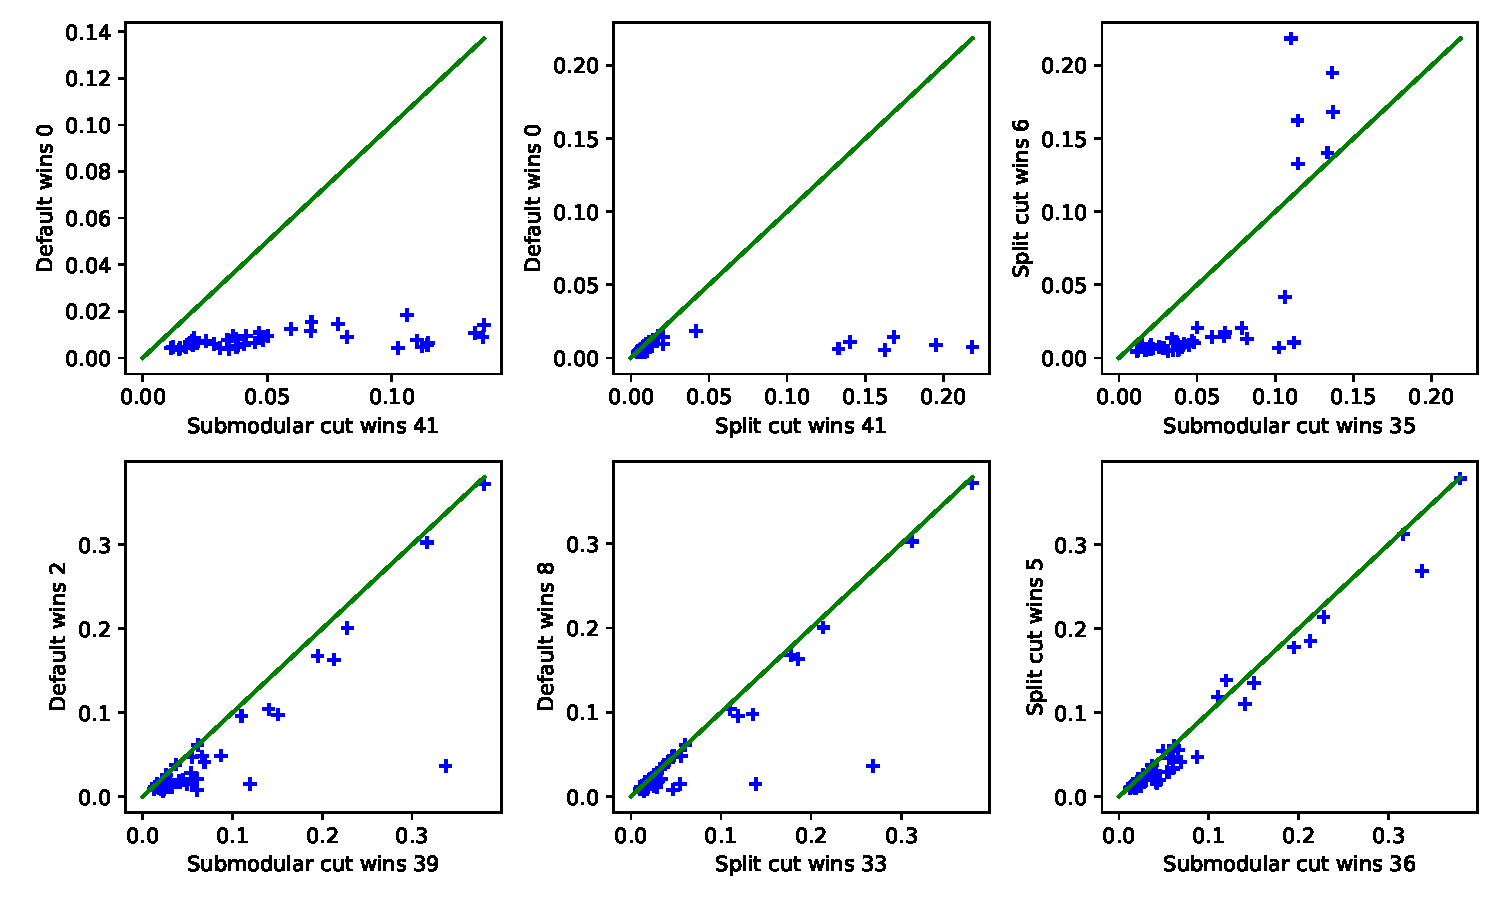
\includegraphics[width=0.99\textwidth]{Chaptersub/media/scatter_mubo.pdf}
    \caption{Scatter plots of \pbm results in standalone (top) and embedded (bottom) configurations}
    \label{fig:mubo}
\end{figure}

\textbf{Experiment 3:} \bdopt.
As mentioned before, the \bdopt problem has a submodular maximization form \eqref{eq.optimal2}. In particular, we can encode it as an extended formulation \eqref{ref.dopt} in \scip. \scip generates gradient cuts for this convex MINLP. Therefore, we can obtain LP relaxations and simplicial conic relaxations.

 Our benchmark consists of two sub-benchmarks.  Recall that the binary vector $x$ selects a subset of $\{M_j \t{M_j}  \in \bS^m\}_{j \in [n]}$, and the information matrix $M(x)$ in \eqref{eq.optimal2} is the sum of matrices in the selected subset. Thus, the problem data of \eqref{eq.optimal2} are variable dimension $n$, matrix size $m$, cardinality number $k$, and matrices $M_j \t{M_j}$.  We next outline the procedure for generating them.
 
The first sub-benchmark consists of 15 block design  instances. We follow the method in \cite{sagnol2015computing} to generate these instances.  Let $x:=(x_{1,2},x_{1,3},\dots,x_{1,m+1},\dots,x_{m,m+1}) \in \{0,1\}^n$, where $n =\binom {m+1} 2$. Let  $H(x)$  be an undirected graph  with $m+1$ vertices. If $x_{i,i'} =1$, there is an edge between vertices $i,i'$; otherwise, no edge 
connects them. We have $M(x) = P L(x)\t P$, where $L(x) := \sum_{i,i'} x_{i,i'} (\mathbf{1}_i - \mathbf{1}_{i'} ){(\mathbf{1}_i - \mathbf{1}_{i'})} ^{\top} \in \bS^m \subseteq \bR^{m \times m}$ is
the Laplacian of $H(x)$, and $P \in \bR^{m \times (m+1)}$ is the matrix
that transforms an $(m+1)$-dimensional vector $v$ to the vector obtained by keeping the first
$m$ entries of $v$.  In other words, $M(x)$ is the submatrix of the Laplacian of $H(x)$
obtained by removing its last row and last column. Then an optimal solution to \eqref{eq.optimal} corresponds to the graphs with $n$ nodes and $k$
edges that have a maximum number of spanning trees. Note that  $M_j =  P  (\mathbf{1}_i - \mathbf{1}_{i'} )\in \bR^{m \times 1}$ is a single-column matrix, which  is degenerated to a $m$-dimensional vector.  We generate a block design instance for each combination of $m \in \{10, 11, 12\}, n =\binom {m+1} 2, k \in \{m, m+1, m+2, m+3, m+4\}$. This results in a total of 15 combinations.

The second sub-benchmark consists of 30 random Gaussian instances. We generate a Guassian instance for each combination of \[(n,m) \in \{(50,20),(50,30),(60,24),(60,36),(70,28),(70,42)\}\] and \[k \in \{m,m+1,m+2,m+3,m+4\}.\] This results in a total of 30 combinations. We still let each $M_j$ be a single-column matrix (\ie a vector), and its entries  are drawn from a Gaussian distribution with zero mean  and  a variance of $1/\sqrt{n}$. 



We set the regularization constant $\epsilon $ to $10^{-6}$. \scip can find  primal feasible solutions at the root node using its internal heuristics. We select the best primal bound given by these solutions among all settings as the reference primal bound.  Since \scip's internal gradient cuts are important for linearizing convex nonlinear constraints, we  keep the gradient cuts but disable all integer-oriented cuts (GMI cuts and mixed-integer rounding cuts etc.) in the standalone configuration.

In \Cref{gamma}, we report the computational results. We divide the results of block design and Gaussian random instances, since the density of  matrices are different. Looking at the default setting in different benchmarks, there is  no difference between the standalone and embedded configurations in terms of the closed root gap. This means that integer-oriented cuts do not improve the root node LP relaxations. We see the same problem for intersection cuts, which do not close the root gap but increase the computing time.  In particular, the number of separated cuts is around one. Thereby, many intersection cuts are too weak to add to the cut pool.

We recall that  intersection cuts and many integer-oriented cuts are LP-based cuts, \ie derived from an LP relaxation of  the extended formulation \eqref{ref.dopt}. Therefore, their strengths depend on the LP relaxation.  Based on the types of MINLPs, there are two basic ways to construct initial LP relaxations.  For nonconvex MINLPs, one way usually uses the factorable programming and term-wise envelopes \cite{mccormick1976computability}. Notable examples are Boolean multilinear constraints and  continuous quadratic constraints \cite{munoz2020maximal}.  The McCormick envelopes or Boolean linearization techniques are used to construct their LP relaxations, which have a finite number of constraints.  


For convex MINLPs, the other way linearizes nonlinear constraints, and the number of constraints in the LP relaxation can grow to infinity. This is because  a convex nonlinear constraint is equivalent to an infinite number of linear constraints.  Given that \scip may incorporate numerous gradient cuts to approximate the convex MINLP \eqref{ref.dopt}, we can better understand its behavior in a simplified scenario. Consider a smooth convex body approximated by a polyhedral outer approximation, where each vertex and its associated faces define one or several simplicial cones, representing optimal tableau cones. As the polyhedron closely approximates the convex body, the vertex comes closer to the border manifold of the convex body, and the simplicial cones approach the tangent space of the manifold at that vertex. Consequently, the cones become very flat, and in the most extreme case, they turns into a hyperplane defining the tangent space. When a hyperplane intersects an $\cS$-free set, this results in the hyperplane itself. Therefore, it is highly likely that our separators will generate weak intersection cuts. In summary, the weakness of intersection cuts is due to the flatness of the optimal tableau cone.

\begin{table} [htbp]
\centering
\scalebox{0.71}{
\begin{tabular}{c|c|cr|cccr|cccr}
\toprule
\multirow{2}{*}{\texttt{Benchmark}} & \multirow{2}{*}{\texttt{Configuration}} &
\multicolumn{2}{c|}{\texttt{Default}}    &
\multicolumn{4}{c|}{\texttt{Submodular cut}} &
\multicolumn{4}{c}{\texttt{Split cut}} 	 \\
 & & closed & time & closed & relative & time & cuts & closed & relative & time & cuts\\
\hline
 \multirow{2}{*}{\texttt{Block design}} & standalone &  0.59 & 20.46 & 0.59 & 1.0 & 18.71 & 1.84 & 0.59 & 1.0 & 11.62 & 1.77  \\
  &  embedded & 0.59 & 21.44 & 0.59 & 1.0 & 19.0 & 1.84 & 0.59 & 1.0 & 12.41 & 1.77 \\
  \hline
 \multirow{2}{*}{\texttt{Gaussian}}  &  standalone  &  0.83 & 213.13 & 0.83 & 1.0 & 415.07 & 1.45 & 0.83 & 1.0 & 214.17 & 1.45 \\
& embedded  &  0.83 & 214.77 & 0.83 & 1.0 & 426.33 & 1.45 & 0.83 & 1.0 & 214.14 & 1.45 \\
\hline
 \multirow{2}{*}{\texttt{All}}  &  standalone  &   0.75 & 98.47 & 0.75 & 1.0 & 149.54 & 1.57 & 0.75 & 1.0 & 82.6 & 1.55 \\
& embedded  &   0.75 & 100.47 & 0.75 & 1.0 & 153.01 & 1.57 & 0.75 & 1.0 & 84.31 & 1.55 \\
\bottomrule
\end{tabular}}
\caption{Summary of  \bdopt results}\label{gamma}
\end{table}

\begin{figure}[h]
    \centering
    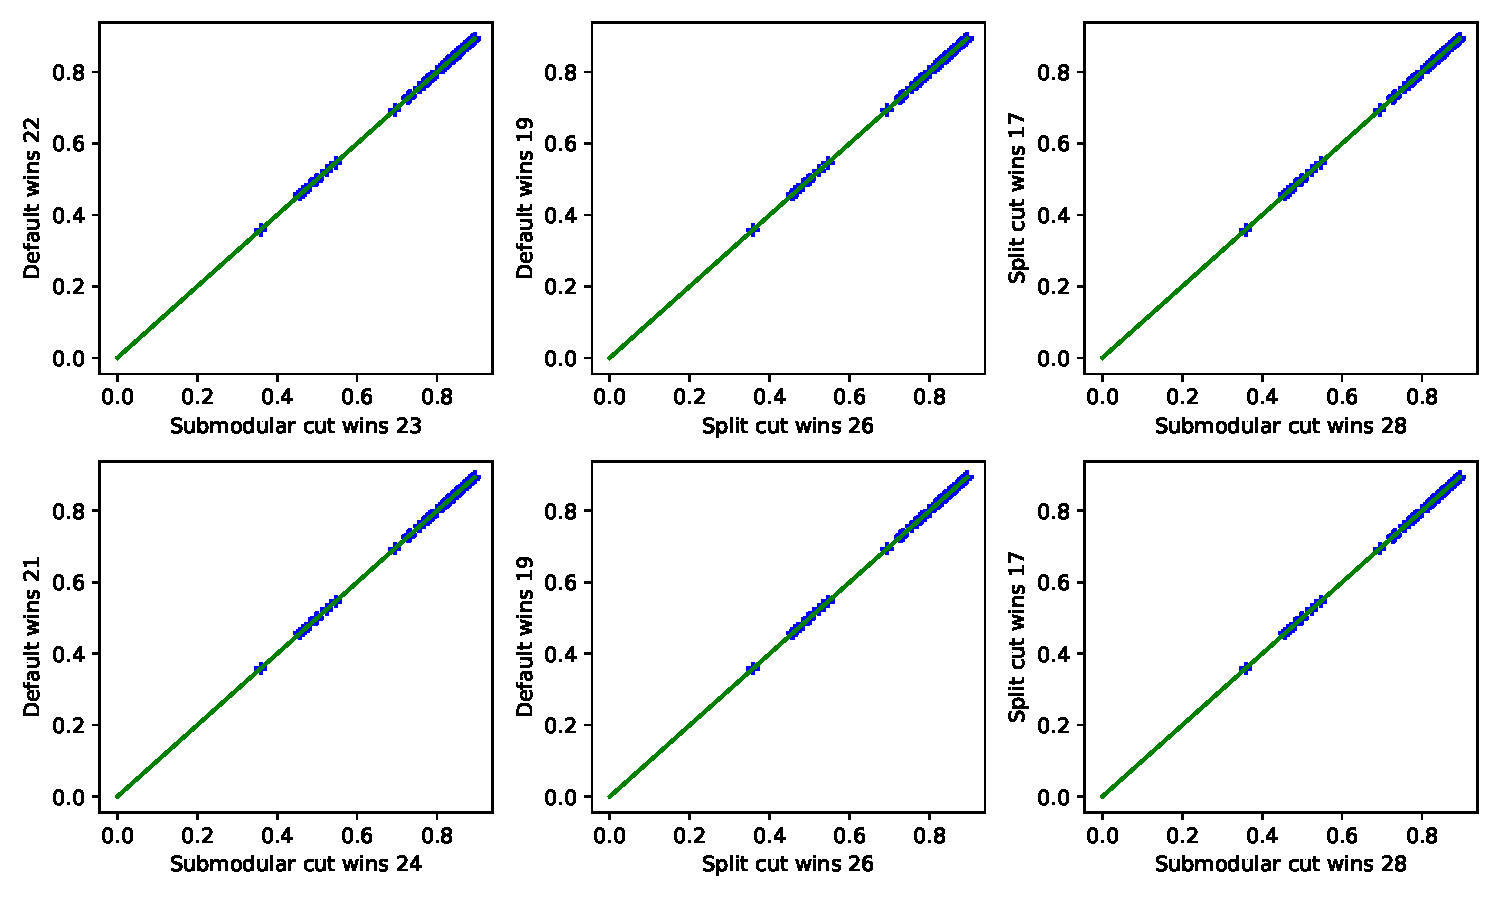
\includegraphics[width=0.99\textwidth]{Chaptersub/media/scatter_dopt.pdf}
    \caption{Scatter plots of \bdopt results in standalone (top) and embedded (bottom) configurations}
    \label{fig:dopt}
\end{figure}



\subsection{Supplementary branch-and-bound computational results}
\label{sec.appb}
We also have an additional branch-and-bound test for \maxcut problem instances in \Cref{sec.cresult}. This test was designed to assess the performance and properties of our cuts in a "production-level" environment, which presents more complex challenges compared to the root node experiment. As such, the parameter settings and analysis in this test are more intricate and require a detailed explanation, which we provide below.

We conducted our tests under the embedded configuration, where the branching rule, node selection rule, and primal heuristics adhere to \scip's defaults. We made adjustments to some parameters specifically to control the behavior of our cut separators in the branch-and-bound algorithm. These parameters are as follows:
\begin{itemize}
	\item SEPA\_FREQ:  the default frequency for separating cuts. We set it to 0, meaning that our cut separators are called at the root node.
	\item SEPA\_NCUTSLIMITROOT: the limit for the number of cuts generated  at the root node. We  set it to 60.
	\item SEPA\_MAXBOUNDDIST: the default maximal relative distance from the current node's dual bound to primal bound compared to the best node's dual bound for applying separation. We set it to 1, meaning that separation is applied at all search nodes.
\end{itemize}


Due to the substantial number of parameter combinations, tuning the parameters for the branch-and-bound test is more challenging compared to the root node experiment. For instance, \scip's internal Gomory mixed-integer cut separator \cite{BibEntry2023Jul2,cornuejols2013safety} is limited to applying at most 30 cuts at the root node, while \scip's quadratic intersection cut separator \cite{BibEntry2023Jul3,chmiela2022implementation} employs at most 20 cuts at the root node and 2 cuts at each non-root node.


In a preliminary branch-and-bound test, we find  that even the default setting can solve the ``pw'' instances of density 0.1 within 100 seconds, while all settings run 3600  seconds on the other instances. To have an unbiased result, we remove ``pw'' instances of density 0.1 and create a sub-benchmark called \maxcut-sub.


For the following branch-and-bound test, we measure the closed duality gap (abbreviated as gap), the relative improvement of the closed duality gap to the default setting, the number of search nodes (abbreviated as nodes), and the number of applied cuts.

\begin{table} [htbp]
\centering
\scalebox{0.85}{
\begin{tabular}{c|cr|cccr|cccr}
\toprule
\multirow{2}{*}{\texttt{Benchmark}} &
\multicolumn{2}{c|}{\texttt{Default}}	&
\multicolumn{4}{c|}{\texttt{Submodular cut}} &
\multicolumn{4}{c}{\texttt{Split cut}}      \\
 & gap & nodes & gap & relative & nodes & cuts & gap & relative & nodes & cuts\\
\hline
 \maxcut-sub  &  0.605 & 231372 & 0.596 & 0.981 & 220176 & 59.87 & 0.618 & 1.026 & 207078 & 42.2\\
\bottomrule
\end{tabular}}
\caption{Summary of \maxcut-sub results in the embedded branch-and-bound test}\label{Aalpha}
\end{table}

Our observations indicate that the submodular cut setting performs slightly worse than the default setting, while the split cut setting performs marginally better than the default setting. As shown in \Cref{fig:qubo3}, the difference in closed duality gaps between the submodular/split cut and default settings is no more than 2\%.
This shows that the optimization landscape of \maxcut problems is very complicated. As for our parameter settings, intersection cuts cannot have a significant impact on the branch-and-bound algorithm.




In contrast to the results in the root node experiment, we find that the split cut setting outperforms the submodular cut setting in the branch-and-bound test. Detailed cut information obtained during debugging reveals that the condition number of submodular cuts can be thousands of times larger than that of split cuts, and the submodular cuts can be denser as well. Consequently, these numerical properties make the submodular cuts less stable and efficient compared to the split cuts.

When considering the approximation of the Boolean-hypograph $\hyp_{\cB}(g)$, where $g$ represents any function over $\cB$, we can deduce from \Cref{thm.bin} that the splits define a class of maximal Boolean-hypograph-free sets. Although the split cuts are independent of  the values of $g$,  we can use the split cuts to approximate the Boolean-hypograph of $g$.  While one can find other Boolean-hypograph-free sets based on the values of $g$, the resulting cuts will likely exhibit the same numerical properties as our submodular cuts.

As a result, future research should consider this finding when exploring intersection cuts. However, it is also worthwhile to investigate the performance of submodular cuts in other problems and algorithms, such as \pbm problems and the diving heuristic.






\begin{figure}[h]
    \centering
    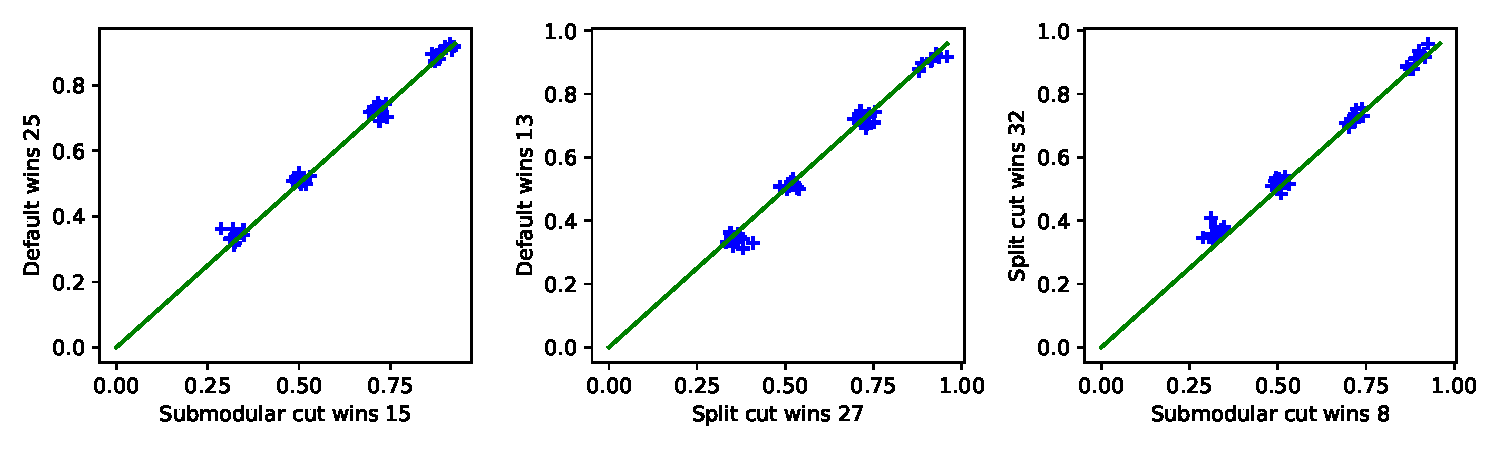
\includegraphics[width=0.99\textwidth]{Chaptersub/media/scatter_qubo_bc.pdf}
    \caption{Scatter of \maxcut-sub results in the embedded branch-and-bound test}
    \label{fig:qubo3}
\end{figure}

\section{Conclusion}\label{sec13}

We construct Boolean-hypograph-free sets for  submodular functions. Our construction relies on a new continuous extension of submodular functions. We characterize maximal Boolean-hypograph-free sets, and generalize our results to sets involving submodular-supermodular functions. These yield intersection cuts for Boolean multilinear constraints. We exploit the submodular structure in an extended formulation of the \dopt problem. We propose a hybrid discrete Newton algorithm that can compute intersection cuts efficiently and exactly. The computational results show that intersection cuts derived from the submodularity are better than those derived from  split cuts for \maxcut and \pbm problems in the root-node experiments. For convex MINLPs, our computational results on the \bdopt problem suggest that  simplicial conic relaxations given by  gradient cuts can be flat, which makes intersection cuts weak.

%As for future studies, an open question is how to extend our methods for discrete submodular functions on general lattices \cite{bach2019submodular} or constrained DR submodular functions \cite{yu2022constrained}. This will result in intersection cuts for integer multilinear constraints  or other discrete nonconvex sets. Another direction is to study the maximal Boolean-hypograph-free sets that enlarge the extended envelope epigraph $\ee{f}$. This study may require additional structural information on submodular functions. We recall that the lifting procedure \cite{ahmed2011maximizing,shi2022sequence} for the base inequalities \cite{Nemhauser1988} only exists for a special class of submodular functions.
%Therefore,  one may only construct  maximal Boolean-hypograph-free sets enlarging $\ee{f}$ for  some special class of submodular functions. This may lead future studies to concrete examples with additional structures, unlike the general submodular function studied in this chapter. A possible strengthening of intersection cuts can use the monoidal technique \cite{ChmielaMunozSerrano2023} or the negative ray extension \cite{chmiela2022implementation}. Constructing intersection cuts from a non-polyhedral corner relaxation is an important open question for convex MINLPs.



%%===========================================================================================%%
%% If you are submitting to one of the Nature Portfolio journals, using the eJP submission   %%
%% system, please include the references within the manuscript file itself. You may do this  %%
%% by copying the reference list from your .bbl file, paste it into the main manuscript .tex %%
%% file, and delete the associated \verb+\bibliography+ commands.                   		 %%
%%===========================================================================================%%


